\documentclass[conference]{IEEEtran}
\usepackage{graphicx}
\usepackage{booktabs}
\usepackage{amsmath}
\usepackage{xurl}
\usepackage[hidelinks]{hyperref}
\makeatletter
\newcommand{\linebreakand}{\end{@IEEEauthorhalign}\hfill\mbox{}\par\mbox{}\hfill\begin{@IEEEauthorhalign}}
\makeatother

\begin{document}

\title{Chhaap: Layout-first diffusion with symbol survival checks for Warli-inspired product design}

\author{\IEEEauthorblockN{Keshav Shetshringi}
\IEEEauthorblockA{Pimpri Chinchwad College\\
of Engineering, Pune, India\\
keshav.shetshringi23@pccoepune.org}
\and
\IEEEauthorblockN{Aadi Kanchankar}
\IEEEauthorblockA{Pimpri Chinchwad College\\
of Engineering, Pune, India\\
aadi27082005@gmail.com}
\and
\IEEEauthorblockN{Swapnil Khillare}
\IEEEauthorblockA{Pimpri Chinchwad College\\
of Engineering, Pune, India\\
swapnil.khillare23@pccoepune.org}
\linebreakand
\IEEEauthorblockN{Pratham Kolettiwar}
\IEEEauthorblockA{Pimpri Chinchwad College\\
of Engineering, Pune, India\\
pratham.kolettiwar23@pccoepune.org}
\and
\IEEEauthorblockN{Prof. Pallavi Nikumbh (Dhade)}
\IEEEauthorblockA{Dept. of Computer Science and Engineering (AI \& ML)\\
Pimpri Chinchwad College\\
of Engineering, Pune, India\\
pallavi.dhade@pccoepune.org}}

\maketitle

\begin{abstract}
Printed Warli products need structured layouts, designed colour and, for repeats, tiles without a visible join, and buyers rarely learn what the motifs mean. Chhaap is a local design tool that turns a short brief into a finished product design. A planner maps the brief to a validated plan, a layout engine places symbols from a sourced lexicon of 25 motifs at product size in one of four templates, colour comes from the layout's layers, and Stable Diffusion 1.5 with a scribble ControlNet and a Warli LoRA only paints the line work. A survival check compares each placed symbol with the output and repairs losses by rerunning with a stronger ControlNet and then by restoring the vector symbol. Over 16 hand-painted pages (852 symbols) diffusion kept 0.587 of hero and support symbols on its first pass; repair raised this to 1.000 at a cost of 141.164 seconds per page on a laptop CPU, against 0.152 seconds for the vector-only rendering. Symbols with more drawing primitives were lost more often ($\rho = -0.474$, $p = 0.0349$), and in a post-hoc test rotated ring dancers survived far less often than upright symbols (0.468 against 0.828). Structured templates spread ink more evenly than random scatter, though the medallion's advantage came from its fillers. An earlier tiling ablation found that circular padding removes the framing a style adapter learns from whole paintings. The human studies were not run.
\end{abstract}

\begin{IEEEkeywords}
latent diffusion, ControlNet, tileable textures, cultural heritage, Warli
\end{IEEEkeywords}

\section{Introduction}

Warli painting comes from the Warli community of the north Konkan coast of Maharashtra. Its figures are drawn in white rice paste on a red ochre wall: people as two triangles joined at the tip, the sun and moon as circles, a sacred square called the chauk at the centre of ritual paintings \cite{dsource_warli,wiki_warli}. The style now reaches buyers mostly as printed goods: textiles, phone cases, wallpaper. Printing an all-over pattern by machine needs a tile whose right edge continues into its left edge and whose top continues into its bottom. A designer working by hand can draw such a tile. A general text-to-image model, asked for "a Warli pattern", usually cannot: the output has a frame of cut-off figures, and repeating it shows a grid of seams.

A second problem sits in the motifs. Warli symbols carry meanings that the community and its documenters have recorded, and a buyer who sees a printed tarpa dance has no way to learn what it is. If a model generates the picture first and a captioner guesses its symbols afterwards, any explanation printed with the product can be wrong.

Chhaap reverses the order. A composer places symbols from a sourced lexicon on a toroidal canvas, draws them as a black and white control image, and records which symbol went where. Stable Diffusion 1.5 then paints the style over that layout through a ControlNet, with circular padding in every convolution so that the tile wraps. The meaning card is filled from the lexicon rows of the placed symbols, so it is correct by construction, within the limits of its sources.

A second version turns this tile generator into a product design tool. Published Warli prints are organised into bands, rings and medallions with borders and fillers; colour is designed in three to five tones; and the product decides the layout. In this version a layout engine owns structure and colour, diffusion only supplies the hand-painted line, and a survival check confirms that every important symbol is still present before the design is shown.

This paper reports a working, local version of both, run on a laptop CPU. Its contributions are:
\begin{itemize}
\item a sourced symbol lexicon of 25 Warli motifs, each with a drawable geometric recipe and a public source URL, and a provenance manifest format for the training images;
\item a compose-then-stylize pipeline whose meaning cards are true by construction;
\item a layout engine with four templates, layered colour and product-specific layouts, and a per-symbol survival check with repair, together with a measurement of which symbols diffusion loses;
\item a seam metric, the Seam Discontinuity Ratio (SDR), a tiling ablation, and an account of where the metric fails on sparse tiles;
\item a local, open tool that shows each generative stage;
\item a proposed licensing model for deployment, in which Warli artists license a style adapter for royalties. It has not been tested.
\end{itemize}
We use "seamless" in its texture-synthesis sense: a tile is seamless when its repeat shows no visible join.

\section{Related work}

\textit{Latent diffusion and adaptation.} Latent diffusion models run the denoising process in the latent space of an autoencoder, which made 512-pixel text-to-image generation affordable \cite{rombach2022ldm}. Stable Diffusion 1.5 is the public model of that family we build on. LoRA adapts a large network by learning a low-rank update to frozen weight matrices \cite{hu2022lora}; the same idea is now the usual way to teach a diffusion model a style from a few hundred images. DreamBooth fine-tunes the whole model on a handful of subject images bound to a rare token \cite{ruiz2023dreambooth}. We use a trigger word in the same way, through LoRA. LCM-LoRA distils a latent consistency model into a LoRA that lets Stable Diffusion sample in 4 to 8 steps \cite{luo2023lcmlora}; it is what makes CPU generation usable here. TAESD is a small distilled autoencoder that decodes latents cheaply enough to preview each step \cite{taesd}.

\textit{Spatial control.} ControlNet attaches a trainable copy of the diffusion encoder to a frozen model and conditions it on an image such as edges, depth or a scribble \cite{zhang2023controlnet}. We use its scribble variant, so the composer's drawing fixes where each figure sits while the base model and LoRA decide how it looks.

\textit{Tileable textures.} The Periodic Spatial GAN builds periodic latent fields so that its outputs tile \cite{bergmann2017psgan}. TileGAN assembles large textures from tiles of a pretrained GAN's latent space \cite{fruhstuck2019tilegan}, and SeamlessGAN trains a discriminator to judge tiling seams directly \cite{rodriguezpardo2022seamlessgan}. Tiled Diffusion generates diffusion outputs that join at their edges, from a single self-tiling texture to many-to-many tile sets and 360-degree images \cite{madar2025tiled}. Chhaap uses a simpler and older community technique, circular padding in every convolution, and measures it with an ablation.

\textit{Evaluation.} FID compares Inception feature statistics of generated and real images \cite{heusel2017fid}. KID replaces FID's Gaussian assumption with a polynomial-kernel MMD estimate that is unbiased, which matters at our sample sizes \cite{binkowski2018kid}. CLIP embeddings \cite{radford2021clip} support zero-shot filters and linear probes; we use both. BLIP generates the training captions \cite{li2022blip}.

\textit{Cultural heritage.} Warli painting has held a Geographical Indication (GI) since 2014 \cite{gi_warli}. GI status for Indian folk art is contested: when Gond painting received its GI in April 2023, Bhopal-based Gond artists and the family of Jangarh Singh Shyam objected to being left off the applicants \cite{pari_gond}. A style adapter trained on scraped images sits inside that dispute, which is why we label every output and propose an artist-licensed adapter.

\section{Data}

\textit{Style images.} We use the Kaggle Indian paintings dataset \cite{kaggle_indian_paintings}, which has eight classes: Gond, Kalighat, Kangra, Kerala mural, Madhubani, Mandana, Pichwai and Warli. Its images were scraped from the web and it states no licence, so we treat it as research-only material and say so in the tool. All eight classes train the style probe of experiment E2. Only Warli trains the LoRA.

The Warli folder held 97 readable images. We removed perceptual-hash duplicates (distance 6 or less; none were found), dropped 17 images whose short side was under 512 pixels, and ran a CLIP zero-shot filter that compared each image against prompts for a Warli painting, a product photograph, a watermarked image and a page of text. The filter removed 2 images. A contact-sheet review then found 22 more that the filter had missed: framed prints photographed on walls, canvas renders, listings with dimensions printed on them, a stock image with a watermark, a craft-kit box and a person posing in front of a mural. Most web images of Warli are product photographs, and a zero-shot filter with four prompts does not separate a painting from a photograph of a painting. The remaining 56 images were centre-cropped to 512 by 512 and split 80/20 with a fixed seed into 45 training and 11 held-out images. The held-out images are never trained on and serve as the reference set for KID. A manifest records, for every image, its class, source, licence status, size, whether it was kept, why it was dropped and its split.

\textit{Symbol lexicon.} The lexicon has 25 rows. Meanings come from six public sources: the Wikipedia article on Warli painting \cite{wiki_warli}, an IIT Bombay D'Source design resource \cite{dsource_warli}, an IGNCA essay \cite{ignca_warli}, an Organiser article \cite{organiser_warli}, Sarmaya museum records \cite{sarmaya_kansari} and a MeMeraki craft blog \cite{memeraki_warli}. These are uneven. The blog is a retailer's page and supplies the meanings of the lagna chauk, the ladder and the five-headed deity, which we could not find in a stronger source. Where a source gives a meaning but no drawing, the visual rule is our own schematic: the tool draws Kansari as a woman holding a grain sheaf, and the row says this drawing is not a documented iconography. We dropped a snake row because its only source linked the snake to the tarpa instrument, not to a snake motif. No Warli artist has checked any row.


\section{Method}

\subsection{Lexicon and composer}

Each lexicon row has an id, a name, a local name where the source gives one, a meaning, a context, a source URL and a \texttt{visual\_rule}. The visual rule is a short drawing program in symbol-relative units (the symbol spans $[-0.5, 0.5]^2$): filled discs and polygons, polylines, rectangles, rays, arcs, and two composition operators, \texttt{use} (draw another symbol, scaled) and \texttt{circle\_of} (draw $n$ copies on a ring). The tarpa dance is therefore a tarpa player inside a ring of 14 human figures, and the human figure is two triangles meeting at the apex with a disc for the head. The composer executes these programs directly, so the lexicon is the only definition of each symbol.

A story is a list of symbol ids with counts. The first symbol is drawn large at the centre; the rest are scattered by seeded rejection sampling with a minimum toroidal distance. Every placement is drawn nine times, shifted by $\{-W, 0, W\} \times \{-H, 0, H\}$, so a symbol crossing an edge reappears on the opposite edge. The composer returns the control image and the list of placed ids. Five stories exist: harvest (Kansari and the tiger god Vaghadevta), wedding (the lagna chauk with Palghata), tarpa dance, village day and forest.

\subsection{Generation}

The text prompt is built from the names of the placed symbols, so text-only and composed conditions ask for the same content. Generation uses Stable Diffusion 1.5 with the ControlNet scribble model, the LCM-LoRA adapter and the Warli LoRA. Circular padding sets \texttt{padding\_mode="circular"} on every 2D convolution in the UNet, the ControlNet, the VAE and the LoRA layers. The latent is then a torus at every resolution of the network, and the decoded tile wraps. Seeds are fixed, and each run writes its prompt, seed, steps, guidance scale, adapter weights, padding flag, placements and per-stage timing to a JSON file.

\subsection{Layout engine}

The first version scattered symbols around one large central symbol. Published Warli products are organised differently: bands of figures, a dance ring, a central square with scenes around it, an all-over field of small motifs, a border, and small fillers so that no ground is left dead. The second version replaces the scatter with a layout engine that works at product size (pixels at 300 DPI) and records every element with its symbol, layer, box, scale and role: hero, support, filler or border. Four templates exist. In the tarpa spiral the tarpa player stands at the centre and dancers hold hands in 2 to 4 concentric rings, each dancer rotated so that its head points outward. In registers, 2 to 4 horizontal bands each carry one story beat, the hero's band taller than the rest, separated by rows of dots. In the medallion, a square frame holds the hero and supporting scenes fill the four quadrants. In the all-over buti, small motifs sit on a half-drop grid. A border kit draws repeating strips of triangles, chevrons, dots, a leaf vine or a chain of dancers around any page.

Sizes follow a fixed hierarchy: the hero is 3 times the support size and 8 times the filler size. Supports never overlap; the check uses oriented boxes, since a ring dancer's axis-aligned box is much larger than the figure. A filler pass then scatters dots, grass ticks, small birds and stars into free space until the ink coverage of the content area reaches a target set by density (0.07, 0.12 or 0.17 for sparse, balanced and dense). Repeating products wrap through a lattice: straight, half-drop or brick. Every element is drawn with its lattice copies, so the tile is periodic by construction, and diffusion runs on the smallest straight-repeating rectangle (twice the tile width for a half-drop) with circular padding. Every stroke receives a small seeded jitter in its width and end points, so even the vector-only rendering does not look ruled.

\subsection{Layered colour and texture}

Colour is designed rather than sampled. Each element belongs to one of five layers: ground, figure ink, accent (the hero, and in dense layouts the triangle bodies of every second figure), border and filler. Eight palettes assign a colour to each layer: white on geru, maroon, indigo or charcoal, and four contemporary sets (mustard, rust and cream; teal, ochre and white; indigo, coral and cream; forest, saffron and ivory). Because the layout knows every element's layer, recolouring is exact. A procedural texture multiplies a blurred noise grain over the ground and lets the ground show through the paint unevenly; it applies to raster files only, and the SVG stays flat.

\subsection{Stylization, survival check and repair}

Diffusion only supplies line quality. The monochrome ink layer is rendered at no more than 768 pixels on its long side, cropped to its drawn area (a blank page margin came back from the model as paper and was then traced as ink), and painted by the same pipeline as before. The output is reduced to two tones, with the ink tone chosen as the one that agrees with the composition. For every placed element we compare composition ink and output ink inside the element's box: both masks are widened by 1 pixel, and the element survives if their intersection over union is at least 0.5. A lost hero or support element triggers a rerun with the ControlNet scale raised by 0.15, at most twice. If it is still lost, the clean vector symbol replaces the output inside its box. Each element records which path it took. The repaired ink is traced with Potrace, and each closed path takes the layer of the element box that covers it most, ties going to the smallest box, so that the hero inside the medallion frame is not coloured as frame. The check measures geometry, not meaning: it cannot see a moon redrawn as a sun inside the marriage square, because the square as a whole still matches.

\subsection{Planner}

A brief such as ``A3 frame for my parents' anniversary, wedding and harvest, maroon and mustard, busy, traditional border'' is turned into a structured plan: product, template, density, repeat, palette, border, hero symbol and up to 4 story beats, each a list of lexicon ids. The plan is validated with a typed schema, and any symbol id that is not a lexicon row is rejected. The default backend is a set of keyword rules. A small local model served by Ollama can replace it when installed, and a hosted model can be called behind an explicit flag; an invalid answer is retried once and then replaced by the rules plan. No backend draws or writes meanings. The plan is shown as an editable card, and a story caption is assembled from the plan and lexicon names; it is discarded if it names a symbol that did not survive.

\subsection{Products}

The product decides the layout. A wall frame (A4 or A3) is one composition with a border and no repeat. A saree set has a body tile on a half-drop, a border strip and a pallu panel, sharing one palette and story. A diary cover is an A5 wrap of back, spine and front. Wallpaper is a half-drop tile, phone wallpapers come in two sizes, and a tee carries a placement print. Print files are drawn at 300 DPI from vectors, the layout itself or the traced stylized ink, and never upscaled. Mockups (a framed print on a wall, a flat saree, a closed and an open diary, a wall section, two phones and a flat tee) are drawn from flat shapes with a perspective warp, and each shows the label.

\subsection{Vectorization and export}

The output is reduced to two tones with Otsu's threshold, taking the lighter class as rice paste and the colours as the class means. Potrace \cite{selinger2003potrace} traces the ink regions into B\'ezier curves, written as an SVG. Large exports (two phone wallpaper sizes and a 4500 by 5400 pixel print file at 300 DPI) are rasterised from these curves with an even-odd fill, so they do not inherit the 512-pixel resolution. Every exported file carries the label ``AI-generated, Warli-inspired. Not a GI-certified Warli painting.''

\subsection{Meaning card}

The card lists each placed symbol once, with its count, local name, meaning, context and source URL, and ends with ``Meanings not yet verified by a Warli artist.'' It is a template over lexicon rows. No language model writes any part of it. In the second version the card is split: symbols that passed the survival check (or were repaired) are listed as present, and symbols that were placed but lost, which can only be fillers or border motifs after repair, are listed separately with a sentence explaining the difference.

\subsection{Seam Discontinuity Ratio}

For a tile $T$ of size $H \times W$ we build the $2 \times 2$ mosaic and compute the Sobel gradient magnitude $G$ of its grayscale. Let $\bar{G}_{\mathrm{seam}}$ be the mean of $G$ in 4-pixel bands centred on the lines $x = W$ and $y = H$, and $\bar{G}_{\mathrm{int}}$ the mean in 4-pixel bands on 8 interior lines (4 vertical, 4 horizontal) drawn with a fixed seed. Then
\begin{equation}
\mathrm{SDR} = \bar{G}_{\mathrm{seam}} / \bar{G}_{\mathrm{int}}.
\end{equation}
An SDR near 1 means the join carries no more edge energy than the rest of the tile. We also report the wrap error: the mean of $|T_{:,0} - T_{:,W-1}|$ and $|T_{0,:} - T_{H-1,:}|$, divided by the mean absolute difference between adjacent interior columns and rows. A unit test checks that a periodic smooth-noise tile scores close to 1 and a shifted tile with a ramp scores well above it.

\section{Experiments}

\subsection{Setup}

All runs used one laptop: an Intel Core Ultra 7 155H CPU with 15 GB of RAM and no usable GPU. On this machine the pipeline samples with LCM-LoRA for 6 steps at 512 by 512 pixels with a guidance scale of 1.0, which needs one UNet pass per step. The ControlNet scale is 0.7. These two values were chosen by eye on seeds 100 and 101, which are outside the evaluation seeds: at a scale of 0.9 the output came out as black ink on a peach ground, while 0.6 to 0.7 with a prompt naming white chalk figures on a red-brown mud wall gave white figures on red ochre. Every condition uses the same 16 seeds (0 to 15), and seed $s$ uses story $s \bmod 5$. The text-only conditions receive the prompt built from the symbols the composer placed for that seed, so every condition asks for the same content.

The Warli LoRA was trained on a free Colab GPU with the diffusers text-to-image LoRA script: rank 16 on the UNet of Stable Diffusion 1.5, 45 training images at 512 pixels, captions from BLIP prefixed with the trigger word \texttt{warli\_style}, batch size 1, learning rate $10^{-4}$, fp16, 1500 steps (34 epochs) with checkpoints every 500. Training took 10.2 minutes. The LoRA is applied at strength 0.8 alongside LCM-LoRA. Its first call on the CPU paid a one-off adapter setup, so an untimed warm-up proof precedes the timed runs.

\subsection{Conditions and metrics}

E1 compares (a) the base model from text only, (b) the base model with circular padding, (c) the LoRA, (d) the LoRA with circular padding and (e) the full pipeline. Each tile is scored with SDR and the wrap error, and (e) is compared with (a) by a Wilcoxon signed-rank test paired by seed. E2 measures style: KID against the 11 held-out Warli images, with the subset size limited by the reference set, and the Warli probability given by a logistic-regression probe on CLIP ViT-B/32 embeddings of all eight dataset classes. The probe never saw the held-out Warli images. E3 asks annotators which requested symbols are present in (a) and (e) images, and E4 is a blind pairwise preference between (a) and (e), asked again after the annotator reads the meaning card of (e). Both run in the tool's study pages. E5 records seconds per image and the peak resident memory of the process. E6 crosses LoRA checkpoints at 500, 1000 and 1500 steps with strengths of 0.4, 0.8 and 1.2.

The second version adds four experiments. E7 stylizes 16 pages, 4 per template, at balanced density (A4 pages; the all-over buti as a half-drop tile), with diffusion seeds from 1000 upward, and records first-pass and final survival for every placed symbol. Complexity is measured as the number of drawing primitives in a symbol's recipe and as its ink share when drawn alone. E9 reuses those runs to compare vector-only rendering, stylization and stylization with repair on survival and time. E8 compares each template with random scatter of the same story symbols over 16 seeds, measuring evenness as the coefficient of variation of ink coverage over a 4 by 4 grid of the content area, with and without fillers, and counting overlapping symbol pairs. E10 runs 20 fixed briefs through each available planner backend and checks automatically how many of the constraints each brief states (product, palette colours, density, story) the plan satisfies. The briefs were written before any planner ran on them, by the same author as the rules backend. Blind preferences for E8 and E9 are collected in the study pages.

\section{Results}

\subsection{E7: which symbols survive diffusion}

Across the 16 pages, diffusion kept 0.583 of support symbols (n = 533), 0.750 of heroes (n = 12) and 0.805 of fillers (n = 307) on its first pass (Fig.~\ref{fig:e7}). Survival depended on the template: 0.512 in the tarpa spiral, 0.763 in the all-over buti, 0.838 in the medallion and 0.877 in registers. We expected complex ritual symbols to be lost first, and the data lean that way. Over the 20 symbols placed at least 3 times, symbols with more drawing primitives survived less often ($\rho = -0.474$, $p = 0.0349$); ink share did not predict survival ($\rho = 0.181$, $p = 0.4459$). The correlation is fragile. An earlier run on layouts with a placement bug (some planned symbols were skipped) showed no correlation, and the plain human figure, with 7 primitives, survived in only 0.412 of 187 placements, while the marriage square, the most complex recipe, survived in both pages that used it.

After seeing this we tested two other explanations, and we report both as post hoc. Drawn size had a weak and non-monotonic effect: first-pass survival by size quartile was 0.607, 0.489, 0.419 and 0.832 ($\rho = 0.137$, $p = 0.0014$). Rotation had a strong one: rotated symbols survived in 0.468 of 365 cases and upright ones in 0.828 of 180 (Fisher's exact test, odds ratio 0.183, $p = 1.51 \times 10^{-16}$). Every rotated symbol is a dancer in a tarpa ring, so rotation is confounded with crowding: the dancers touch hands, and the model tends to merge them into a band. Repair recovered every lost hero and support symbol. Of the 545, 317 passed the first time, 42 were recovered by a rerun with a stronger ControlNet and 186 by restoring the vector symbol. Fillers are not repaired, and 50 of the 307 stayed lost. Ten of the 16 pages used both reruns. Fig.~\ref{fig:e7ex} shows the failure modes: rings of small figures merge into bands and filler dots become stars.

\begin{figure}[t]
\centering
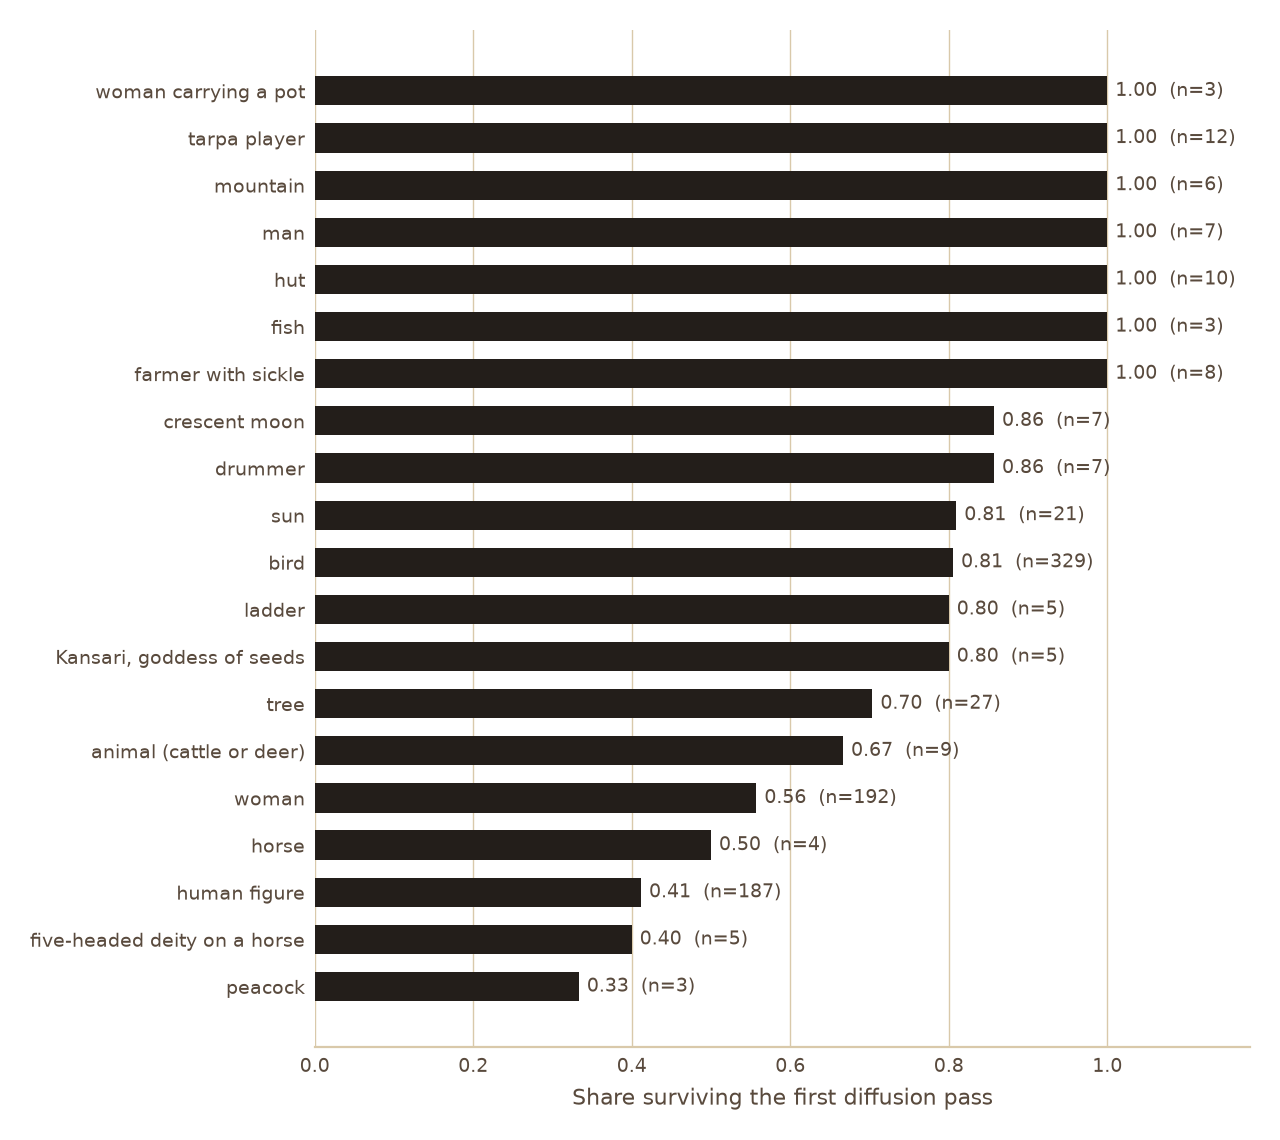
\includegraphics[width=\columnwidth]{../eval/figures/e7_survival.png}
\caption{E7: share of each symbol surviving the first diffusion pass, over 16 pages (symbols placed at least 3 times).}
\label{fig:e7}
\end{figure}

\begin{figure*}[t]
\centering
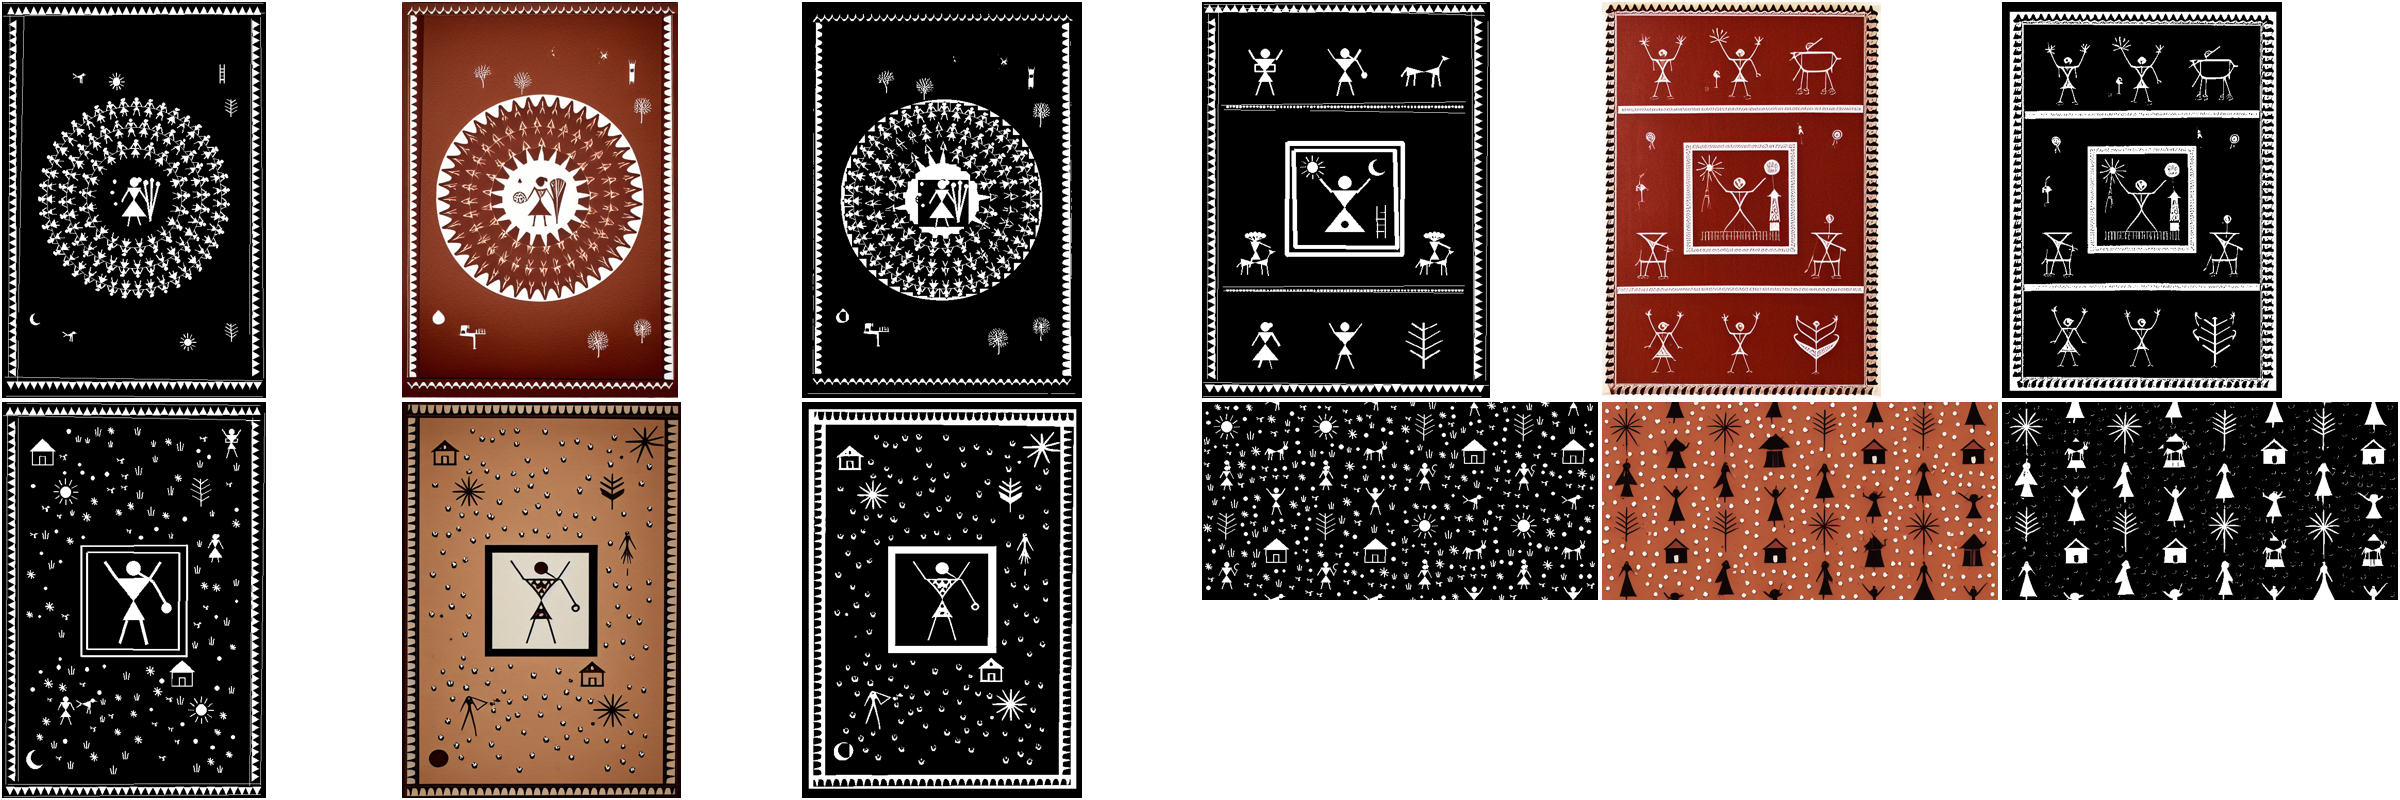
\includegraphics[width=\textwidth]{../eval/figures/e7_examples.png}
\caption{E7, four of the 16 runs. For each run: the composition (control image), the stylized output and the repaired ink. Top: tarpa spiral and registers. Bottom: medallion and all-over buti.}
\label{fig:e7ex}
\end{figure*}

\subsection{E8: structure against random scatter}

\begin{table}[t]
\caption{E8: evenness of ink (coefficient of variation over a 4 by 4 grid, lower is more even), 16 seeds per layout.}
\label{tab:e8}
\centering
\resizebox{\columnwidth}{!}{%
\begin{tabular}{llll}
\toprule
Layout & CV & CV without fillers & Overlapping pairs \\
\midrule
scatter & 1.002 $\pm$ 0.126 & 1.002 $\pm$ 0.126 & 0.125 $\pm$ 0.342 \\
tarpa spiral & 0.826 $\pm$ 0.040 & 0.826 $\pm$ 0.040 & 0.000 \\
registers & 0.470 $\pm$ 0.107 & 0.598 $\pm$ 0.078 & 0.000 \\
medallion & 0.504 $\pm$ 0.119 & 1.028 $\pm$ 0.052 & 0.000 \\
all-over buti & 0.133 $\pm$ 0.029 & 0.322 $\pm$ 0.070 & 0.000 \\
\bottomrule
\end{tabular}}
\end{table}

Every template spread ink more evenly than random scatter of the same symbols (Table~\ref{tab:e8}; Wilcoxon against scatter, $p = 0.0002$ for the tarpa spiral and below $10^{-4}$ for the others), and none placed two symbols over each other. The comparison is not clean, because only the templates run the filler pass, and their pages carry about twice the ink of scatter (0.122 to 0.152 against 0.065). Removing the fillers separates the two effects. Registers and the all-over buti stay more even than scatter on structure alone. The medallion does not: without fillers its coefficient of variation is 1.028, no better than scatter ($W = 54$, $p = 0.4954$), so its evenness comes from the fillers around a large central block. The blind preference between scatter and templates was not run.

\subsection{E9: what diffusion adds}

\begin{table}[t]
\caption{E9: symbol survival and time per page for the 16 E7 pages.}
\label{tab:e9}
\centering
\resizebox{\columnwidth}{!}{%
\begin{tabular}{llll}
\toprule
Rendering & Hero and support & All symbols & Seconds per page \\
\midrule
vector only & 1.000 & 1.000 & 0.152 $\pm$ 0.075 \\
stylized & 0.587 & 0.665 & 67.728 $\pm$ 40.398 \\
stylized + repair & 1.000 & 0.940 & 141.164 $\pm$ 67.535 \\
\bottomrule
\end{tabular}}
\end{table}

Vector-only rendering keeps every symbol by construction and takes a fraction of a second. Diffusion alone loses 0.413 of the hero and support symbols (Table~\ref{tab:e9}). Repair restores all of them and roughly doubles the time, because 10 of 16 pages needed two reruns. What diffusion adds is line quality: uneven strokes, merged rice-paste blobs, the look of paint. None of our metrics measures that, and the blind preference that would (vector only against stylized with repair) was not run. On this evidence diffusion is the most expensive and least reliable stage, and its value is still unmeasured.

\subsection{E10: planner faithfulness}

The rules backend returned a valid plan for all 20 briefs and satisfied 0.944 of their 71 stated constraints: every product and story, 0.889 of the 9 densities and 0.850 of the 20 palettes. Its four misses are informative. No palette contains both maroon and mustard. ``Not too busy'' was read as busy. Crimson and gold are not palette names. In ``the forest at night, white on black'', the word forest matched a palette tag before black did. Because the briefs and the rules came from the same author, this score is optimistic. The local language model and the hosted backend were not run: Ollama is not installed, and the hosted backend uses a paid quota.

\begin{figure}[t]
\centering
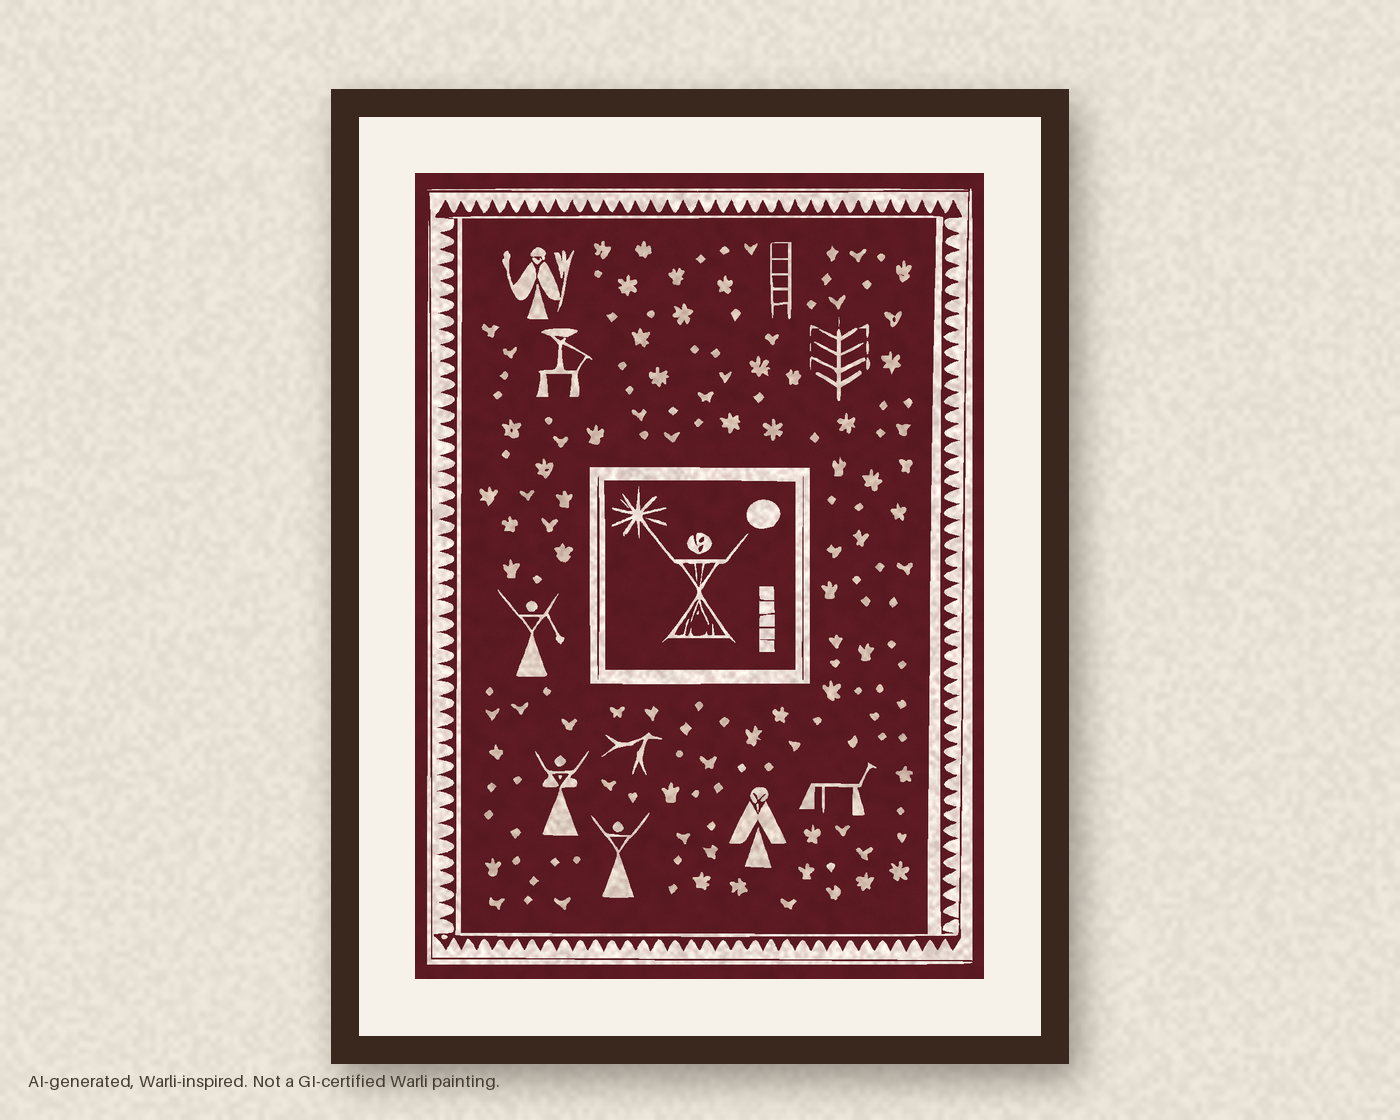
\includegraphics[width=\columnwidth]{../eval/figures/v2_frame_mockup.png}
\caption{The A3 brief from the introduction, hand-painted with repair (design d\_1a1625321af): every hero and support symbol is present.}
\label{fig:frame}
\end{figure}

\begin{figure}[t]
\centering
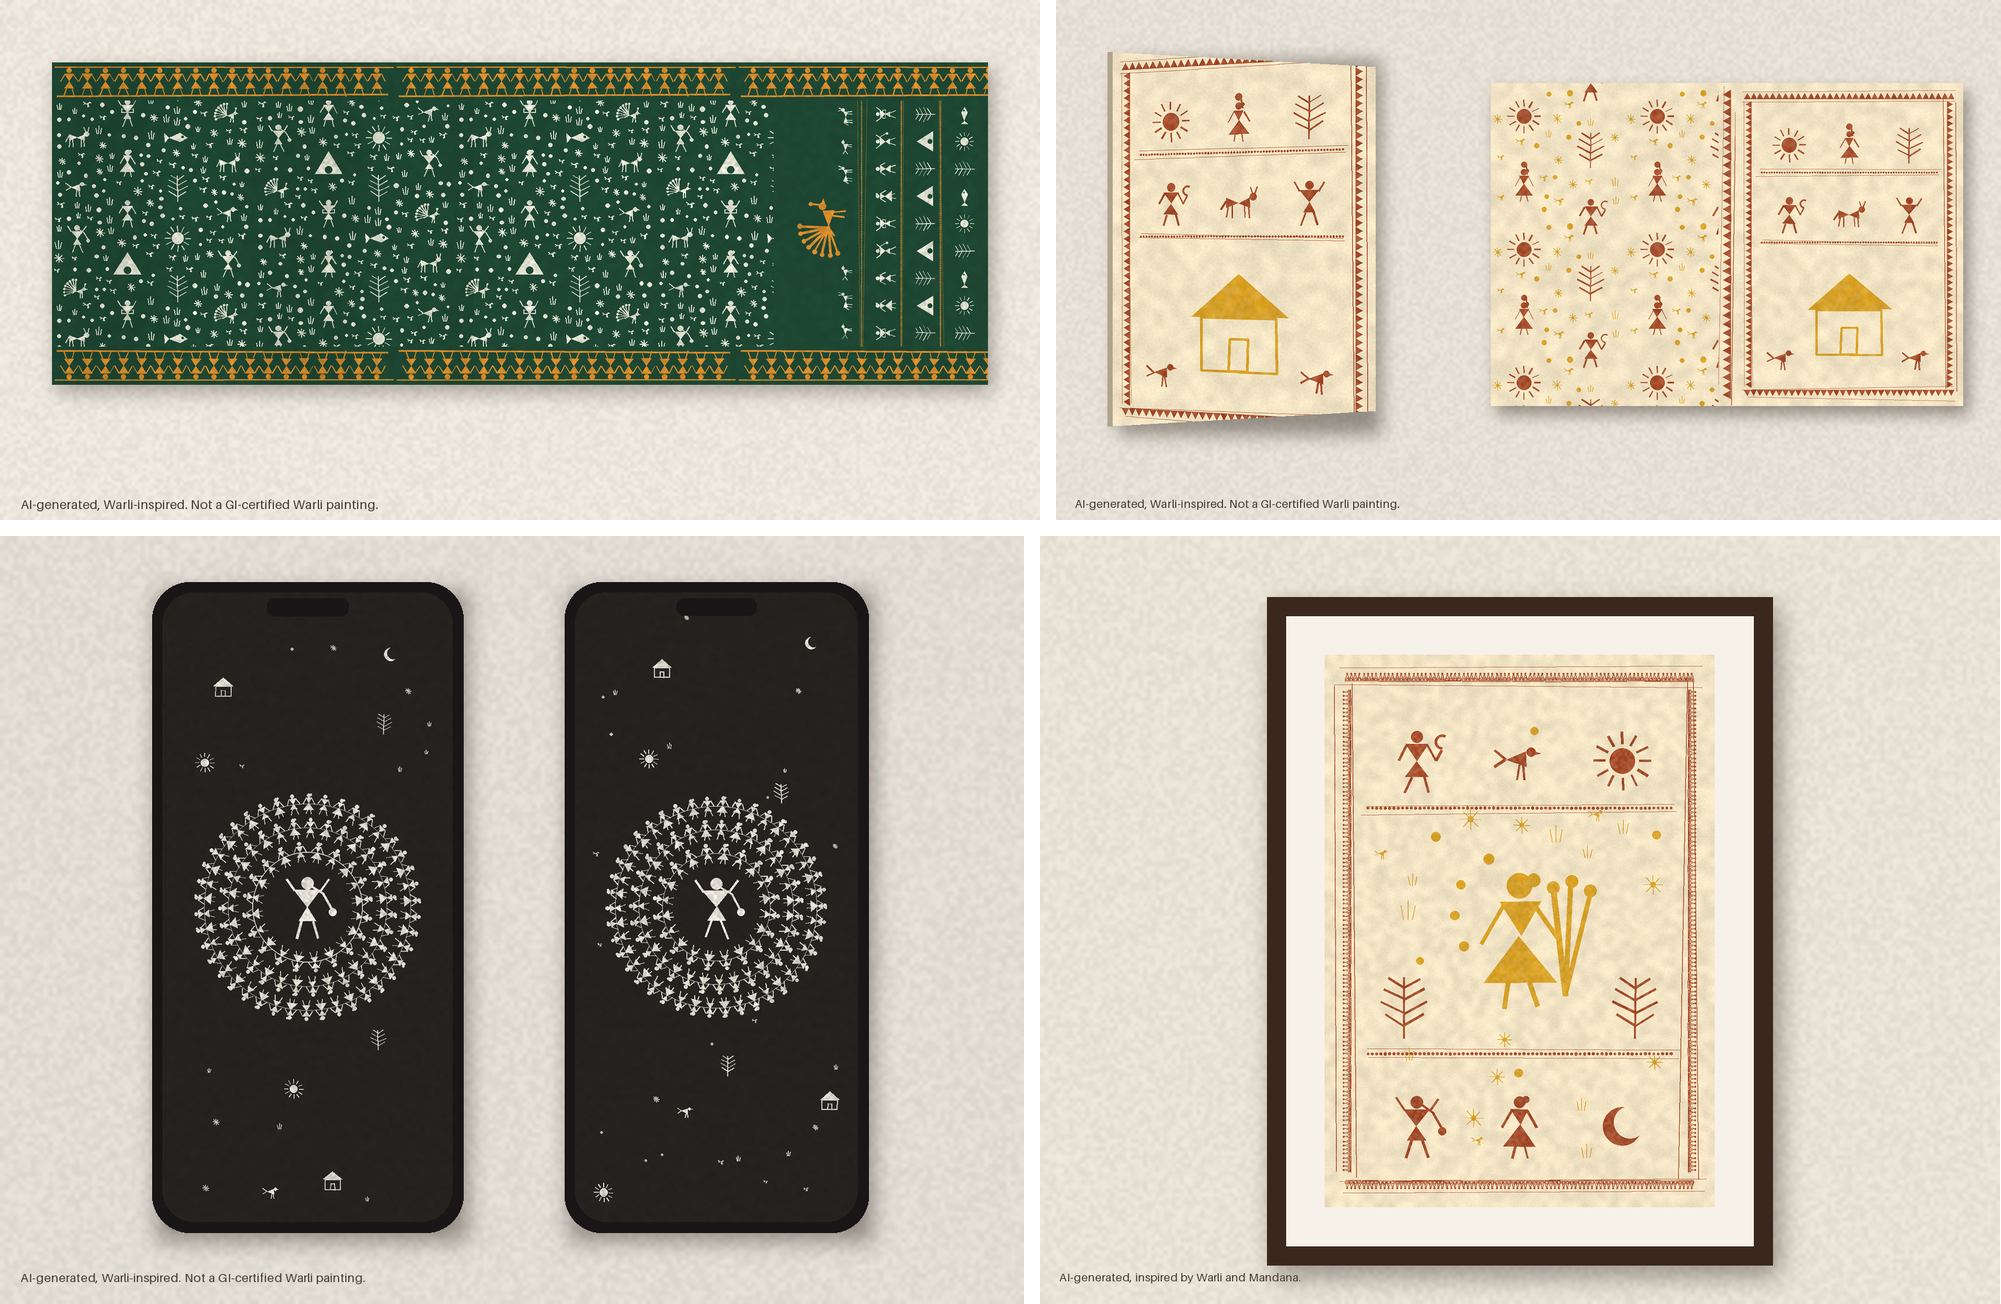
\includegraphics[width=\columnwidth]{../eval/figures/v2_products.png}
\caption{Vector-only designs from four briefs: a saree set, a diary cover, phone wallpapers and a frame that puts a Mandana border around a Warli centre.}
\label{fig:products}
\end{figure}

\subsection{Earlier experiments: the tile generator}

The remaining experiments evaluate the first version, which generates single 512-pixel tiles.

\subsection{E1: tiling}

\begin{table}[t]
\caption{E1 tiling ablation, 16 tiles per condition (mean $\pm$ std).}
\label{tab:e1}
\centering
\resizebox{\columnwidth}{!}{%
\begin{tabular}{llll}
\toprule
Cond. & Pipeline & SDR & Wrap error \\
\midrule
a & text only & 1.008 $\pm$ 0.756 & 1.640 $\pm$ 1.426 \\
b & text + circular & 1.020 $\pm$ 0.184 & 1.004 $\pm$ 0.195 \\
c & text + LoRA & 0.536 $\pm$ 0.625 & 1.190 $\pm$ 2.080 \\
d & text + LoRA + circular & 1.062 $\pm$ 0.192 & 1.060 $\pm$ 0.185 \\
e & full pipeline & 1.018 $\pm$ 0.377 & 1.176 $\pm$ 0.800 \\
\bottomrule
\end{tabular}}
\end{table}

Table~\ref{tab:e1} gives the planned analysis. Apart from (c), every condition has a mean SDR between 1.008 and 1.062, and the Wilcoxon test of (e) against (a) finds no difference (SDR: $W = 50$, $p = 0.375$; wrap error: $W = 58$, $p = 0.632$). The mosaics in Fig.~\ref{fig:mosaics} disagree with that reading. Text-only tiles (a) come out as framed panels, and their $2 \times 2$ repeat is a grid of frames. With the LoRA and no circular padding (c) the framing is stronger: all four tiles shown are a bordered panel or a round medallion, as in the training paintings. With circular padding, (b) and (d) give continuous textures, and the composed tiles (e) repeat without a visible join.

The planned statistic fails because SDR fails in two directions. A broken seam pushes SDR above 1. A framed tile puts a flat border on the seam, and the seam band then has less edge energy than the interior, so SDR falls well below 1: one text-only tile scored 0.24. Averaging over tiles cancels the two. After seeing this we summarised each tile by $|\log \mathrm{SDR}|$, which is 0 for a seamless tile in either direction (Table~\ref{tab:posthoc}). This analysis was defined after inspecting E1, and we report it as post hoc.

\begin{table}[t]
\caption{E1 post hoc: $|\log \mathrm{SDR}|$ (0 is seamless), mean $\pm$ std over 16 tiles, with the planned 8 interior lines and with 64.}
\label{tab:posthoc}
\centering
\resizebox{\columnwidth}{!}{%
\begin{tabular}{llll}
\toprule
Cond. & 8 lines & 64 lines & $0.8 < \mathrm{SDR} < 1.25$ \\
\midrule
a & 0.591 $\pm$ 0.492 & 0.613 $\pm$ 0.442 & 5 of 16 \\
b & 0.130 $\pm$ 0.137 & 0.107 $\pm$ 0.109 & 13 of 16 \\
c & 1.247 $\pm$ 0.937 & 1.207 $\pm$ 0.895 & 2 of 16 \\
d & 0.147 $\pm$ 0.109 & 0.137 $\pm$ 0.090 & 12 of 16 \\
e & 0.279 $\pm$ 0.218 & 0.281 $\pm$ 0.159 & 8 of 16 \\
control images & 0.586 $\pm$ 0.468 & 0.558 $\pm$ 0.444 & \\
\bottomrule
\end{tabular}}
\end{table}

On this statistic circular padding separates clearly from its absence. On the base model, (b) against (a) gives $W = 10$, $p = 0.0013$ with 8 lines. With the LoRA the effect is larger, because the LoRA alone frames more: (c) is the worst condition at 1.247, and (d) against (c) gives $W = 2$, $p = 0.0001$. The full pipeline (e) sits between (a) and (b), at $W = 22$, $p = 0.0155$ against (a) with 8 lines and $W = 17$, $p = 0.0063$ with 64. We expected (e) to match (b) and (d), since its convolutions wrap in the same way. The last row of Table~\ref{tab:posthoc} explains the gap. The composer's control images are seamless by construction, yet they score 0.586, as badly as the framed tiles. A sparse tile has a few figures on a flat ground, and the denominator of SDR depends on whether the random interior lines happen to cross a figure. SDR therefore measures seams reliably only on dense textures such as those of (b). On sparse two-tone tiles it mostly measures where the content fell, and the residual of (e) is lower than that of its own seamless input.

\begin{figure}[t]
\centering
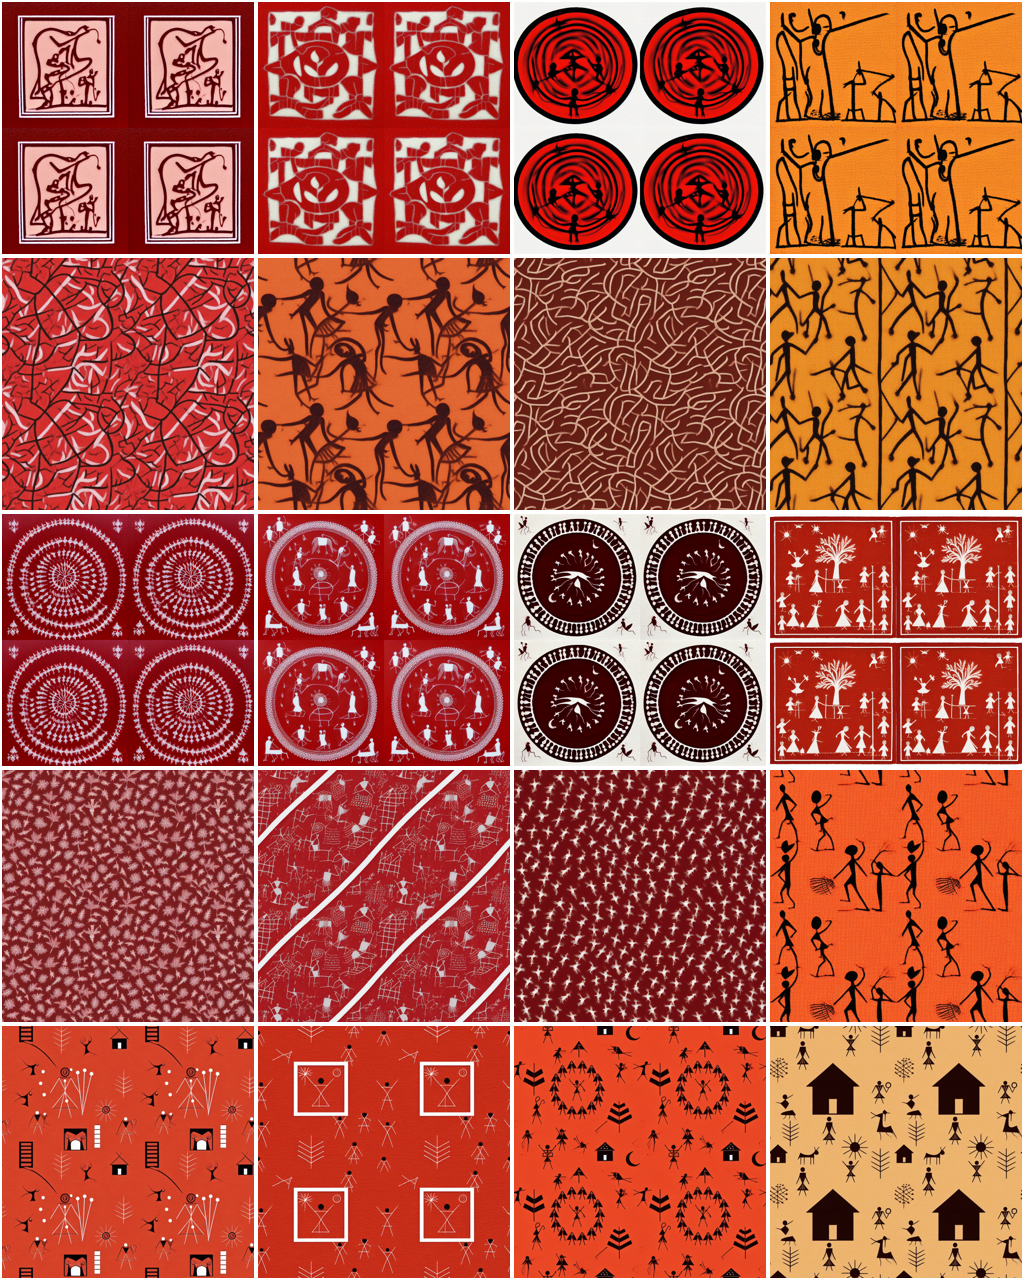
\includegraphics[width=\columnwidth]{../eval/figures/e1_mosaics.png}
\caption{$2 \times 2$ mosaics of four tiles per condition (seeds 0 to 3). Rows from top: (a) text only; (b) text with circular padding; (c) text with the LoRA; (d) text with the LoRA and circular padding; (e) full pipeline. The seam lines run through the centre of each mosaic.}
\label{fig:mosaics}
\end{figure}

\subsection{E2: style}

The CLIP probe reached a test accuracy of 0.806 over eight classes (719 training and 180 test images). On the 11 held-out Warli images it gives a mean Warli probability of 0.301, which sets the scale: the probe is not confident even on real Warli. Base text-only tiles (a) score 0.169, LoRA text-only tiles (c) 0.324 and composed tiles (e) 0.356, the last two at or above the real held-out images. KID agrees for (c), which is the closest to the reference set at 0.024 against 0.067 for (a), but ranks (e) furthest at 0.148. The two metrics measure different things. The scraped reference images are mostly whole framed paintings, dense with figures, and the LoRA learned to produce exactly that, so (c) matches their Inception statistics. The composed tiles are sparse repeats with a few large figures, which CLIP reads as Warli and Inception reads as unlike the reference set. With 11 reference images, KID estimates are also unstable. We do not take either number as a verdict on style, and a low KID here partly rewards the framing that E1 penalises.

\subsection{E3 and E4: human judgements}

Neither study had been run on the final tiles when these results were produced. The annotation page (E3) and the blind preference page (E4) are built into the tool, and the analysis script reads their answers from its database, counting only answers given after the image was generated; a few answers given on an earlier, pre-LoRA set of tiles are therefore excluded. We report both as not run.

\subsection{E5: cost}

\begin{table}[t]
\caption{E5 cost on the test laptop (CPU only), 16 images per condition.}
\label{tab:e5}
\centering
\resizebox{\columnwidth}{!}{%
\begin{tabular}{llll}
\toprule
Cond. & Seconds per image & Denoising (s) & Peak RSS (MB) \\
\midrule
a & 27.710 $\pm$ 0.328 & 20.921 $\pm$ 0.273 & 7383 \\
b & 28.365 $\pm$ 0.372 & 21.290 $\pm$ 0.347 & 7645 \\
c & 27.867 $\pm$ 0.295 & 21.065 $\pm$ 0.246 & 7387 \\
d & 28.469 $\pm$ 0.282 & 21.325 $\pm$ 0.236 & 7646 \\
e & 35.974 $\pm$ 0.262 & 28.778 $\pm$ 0.230 & 7671 \\
\bottomrule
\end{tabular}}
\end{table}

A composed tile takes 36.0 seconds on the laptop CPU (Table~\ref{tab:e5}), of which 28.8 are denoising, against 21.3 seconds of denoising for text with the LoRA and circular padding; the difference is the ControlNet. The LoRA and circular padding each cost little: 27.9 seconds per image for (c) and 28.4 for (b), against 27.7 for (a). The process peaks between 7383 and 7671 MB, most of it the fp32 weights.

\subsection{E6: LoRA steps and strength}

Fig.~\ref{fig:e6} crosses the three checkpoints with three strengths on one composed tile (seed 3, village day). The LoRA changes details: at higher strength and later checkpoints the ground deepens towards orange, and at 1500 steps and strength 1.2 extra figures appear that the composer did not place. It does not change the palette of this tile, which stays black on a pale ground in all nine cells, unlike most composed tiles in Fig.~\ref{fig:mosaics}. SDR on a single sparse tile ranges from 0.776 to 0.983 and, given E1, says little. We kept the final checkpoint at strength 0.8, the setting that adds no unplaced figures.

\begin{figure}[t]
\centering
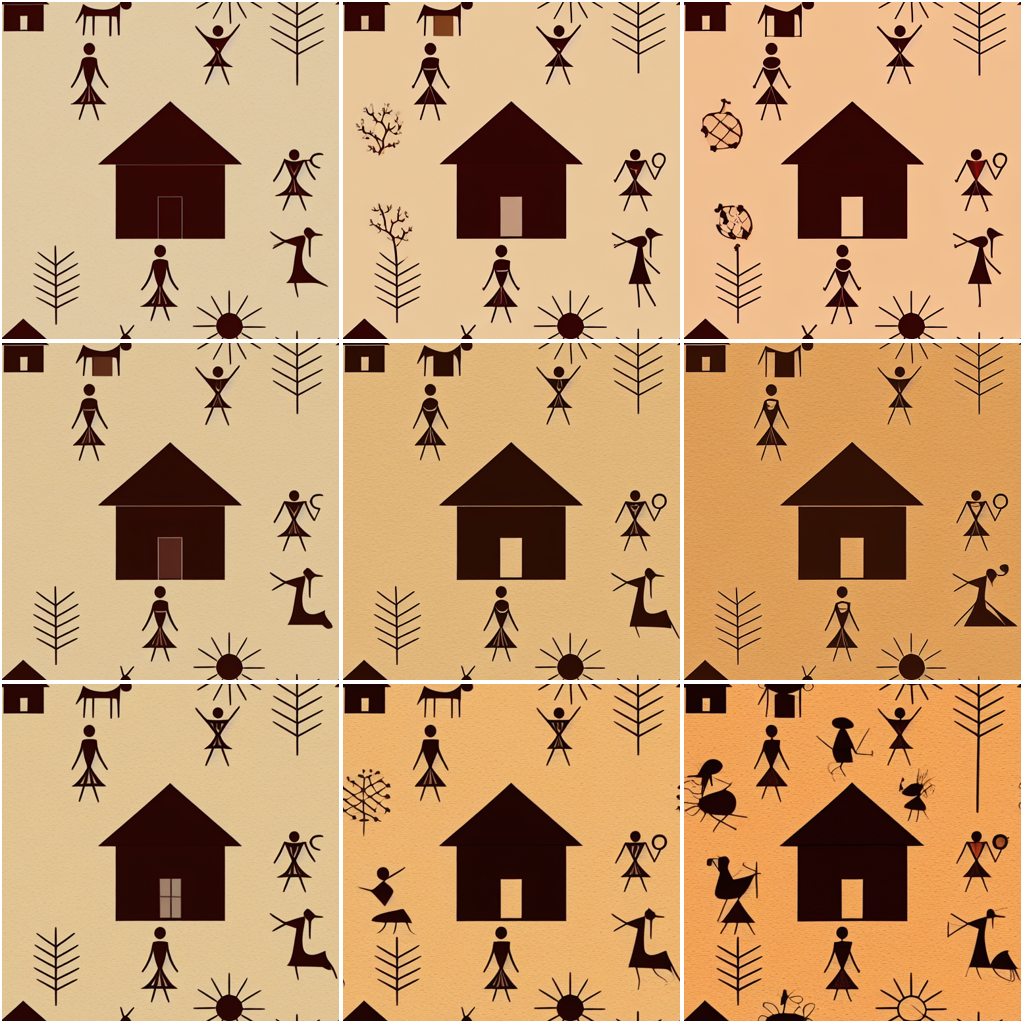
\includegraphics[width=\columnwidth]{../eval/figures/e6_lora_steps_strength.png}
\caption{E6 on seed 3. Rows: LoRA checkpoints at 500, 1000 and 1500 steps. Columns: strength 0.4, 0.8 and 1.2.}
\label{fig:e6}
\end{figure}

\subsection{The tool}

Fig.~\ref{fig:hood} shows the stages of one tile proof: the control image, the six TAESD previews, the decoded tile and its two-tone reduction. In the second version the ``under the hood'' view lays out the same stages for a product design, adding the planner's input and plan, the layout, the survival table with each symbol's path, and the time each stage took. Exports at 4500 by 5400 pixels are drawn from the traced curves; a self-check requires the re-rasterised curves to agree with the two-tone mask on more than 98\% of pixels.

\begin{figure*}[t]
\centering

\includegraphics[width=\textwidth]{../eval/figures/under_the_hood.png}
\caption{One proof, stage by stage (wedding story). From left: composed control image; TAESD previews of the six LCM steps; decoded tile; two-tone reduction used for tracing.}
\label{fig:hood}
\end{figure*}

\section{Discussion}

The second version moved most of the design work out of the model. Structure and colour now come from the layout engine and the palette, and E8 shows that structure alone makes two of the four templates measurably more even than scatter. Diffusion was kept for line quality, and E7 and E9 show its price. Run without a check, it silently drops more than four in ten of the symbols a design is about, and the meaning card would then describe symbols that are not on the print. The survival check makes the card honest again, and repair makes the design complete, but at about twice the time. We cannot yet say whether the hand-painted line is worth that: the blind preference that would decide it was not run. Diffusion lost complex symbols somewhat more often, but the strongest effect was on crowded, rotated small figures. A layout engine can avoid that cheaply, by keeping ring dancers upright or larger, which suggests a design rule rather than a model change.


The clearest result is visual and the metric only half caught it. Circular padding turns text-only output from framed panels into continuous texture, and the composed tiles repeat without seams. The style adapter makes padding more necessary, not less: trained on photographs of whole paintings, the LoRA reproduces their borders and medallions, and only circular padding turns its output back into a repeat. SDR, defined before we saw any output, could not show this on average, because a frame and a break push it in opposite directions, and because sparse tiles make its denominator noisy. The log transform fixes the first problem. The second needs a different reference: comparing the seam band with the same tile shifted by half its width, so that seam and interior carry the same content, would remove the dependence on where figures fall. We have not tested that.

Style metrics disagreed with each other. The CLIP probe placed composed tiles closest to Warli, and KID placed them furthest away while preferring the framed LoRA output. Both rest on small sets (11 reference images for KID), and the reference images are photographs of whole paintings while the outputs are repeat tiles. A style metric for repeat design should compare tiles with tiles, which means building a reference set of real Warli repeats. None exists in this dataset.

The meaning card needs no metric for its own correctness: it lists exactly the symbols the composer placed, by construction. What it cannot guarantee is that the model drew them recognisably. ControlNet at 0.7 keeps the large symbols (the marriage square, the tarpa ring, huts) but small ones can blur into decoration. E3 exists to measure this, and its absence is the largest gap in this paper.

\section{Limitations}

The training images come from a scraped Kaggle dataset with no stated licence. After cleaning, 45 Warli images remain for training and 11 for evaluation, and the held-out set is too small for stable KID. Each condition has 16 samples. The Warli LoRA saw 45 images for 1500 steps, and E6 covers one seed; its effect on palette varies by story, and one story (village day) stayed black on a pale ground. No Warli artist has verified the lexicon, and three of its meanings rest on a retailer's blog. Stable Diffusion 1.5 works at 512 pixels; the print exports are sharp because they are redrawn from vectors, which also reduces each tile to two tones. The human studies had not run, and when they do they will be pilots with one or two annotators. The survival check measures geometry inside each symbol's box: it cannot see a symbol swapped for another inside a composite (a moon redrawn as a sun in the marriage square), and a single ink polarity per image cannot follow a local inversion of figure and ground. E7 used one density and 16 pages, and its explanations of loss are post hoc. The planner was tested only on our own briefs, and only the rules backend ran. The Mandana pack has a sourced lexicon of 14 motifs but no trained adapter, so Mandana designs are painted without one.

\section{Ethics statement}

Warli painting has held a Geographical Indication since 2014 \cite{gi_warli}. A tile from this tool is not a Warli painting, and every exported file says so in its metadata: ``AI-generated, Warli-inspired. Not a GI-certified Warli painting.'' The training data were scraped by a third party without a licence, so we use them for research only. The trained adapter is released with the code for research use under the same caveat, and is not a licence to use the style commercially. Style adapters trained on a community's work take value from that community without its consent. For deployment we propose the opposite arrangement: a LoRA trained on works that Warli artists license for the purpose, with a royalty per generated design paid to the contributing artists. We have not tested this model with artists, and the Gond dispute \cite{pari_gond} shows that deciding who represents a community is itself contested. The meaning card states that no Warli artist has verified its meanings.

\section{Conclusion}

Composing symbols before diffusion makes the explanation of an image a by-product of making it, and circular padding makes the tile repeat. Giving the layout engine the structure and colour, and checking each symbol after diffusion, turns that tile generator into a tool that produces complete product designs whose meaning cards list only what is on the page. Diffusion lost 0.413 of the important symbols on its own, above all rotated dancers in crowded rings, and repair recovered all of them. The measurement side lagged behind: an edge-based seam ratio cannot distinguish a seamless sparse tile from an unlucky one, and the two style metrics disagreed. We leave open whether any automatic metric can judge a repeat design, or whether the judges have to be the people whose craft the design borrows from.

\bibliographystyle{IEEEtran}
\bibliography{refs}

\end{document}
